\subsection{Creating Questions}
Everything in the application that is restricted to admin will only use the Admin.vue component as the view file. In order to start creating questions, the user first need to load the Questions.vue component onto the Admin.vue component. This will call the \$route function in Admin.vue that will you use the vue router to update the path to /admin/questions. This will in return make the Admin.vue load the needed Questions.vue component. The Questions.vue component consist of other components such as EditQuestion.vue, ShowQuestion.vue, SelectCourse.vue and AddQuestionToSession.vue. All components that is related to creating a question can be found in the App/client/components/admin/question folder. On the /admin/questions page there will be a select form to the left, which is in the SelectCourse component. In this select form the user can choose between the available courses in the database. Keep in mind that a course must be chosen for the user to able to create new question. This is done so that a question can immediately be assigned to the given course, since every question should be assigned to at least a course before the question can be allowed to be used in an active session.  If the user attempts to create a question without having a course in the database, an error message will be displayed to the user instead.\\[11pt]
The area in the middle of the Questions component is where the current questions for the selected course is going to be listed. This area has a white background color in contrast with the normal grey background color in order to make it more to noticeable to the user. If there are no questions for the selected course, then this area contains the message “no question.” instead. The Question sends an emit request to the server whenever the component is loaded, the course changes, a question is edited, or a question is created. This emit message will ask server for all the current questions for the current selected course. The server then calls the appropriate select statement in the database and returns the result. The result is then used by the Questions component to update the list of questions. In this way the list should always be up to date with the contents in the database. 
\begin{figure}[H]
	\centering
	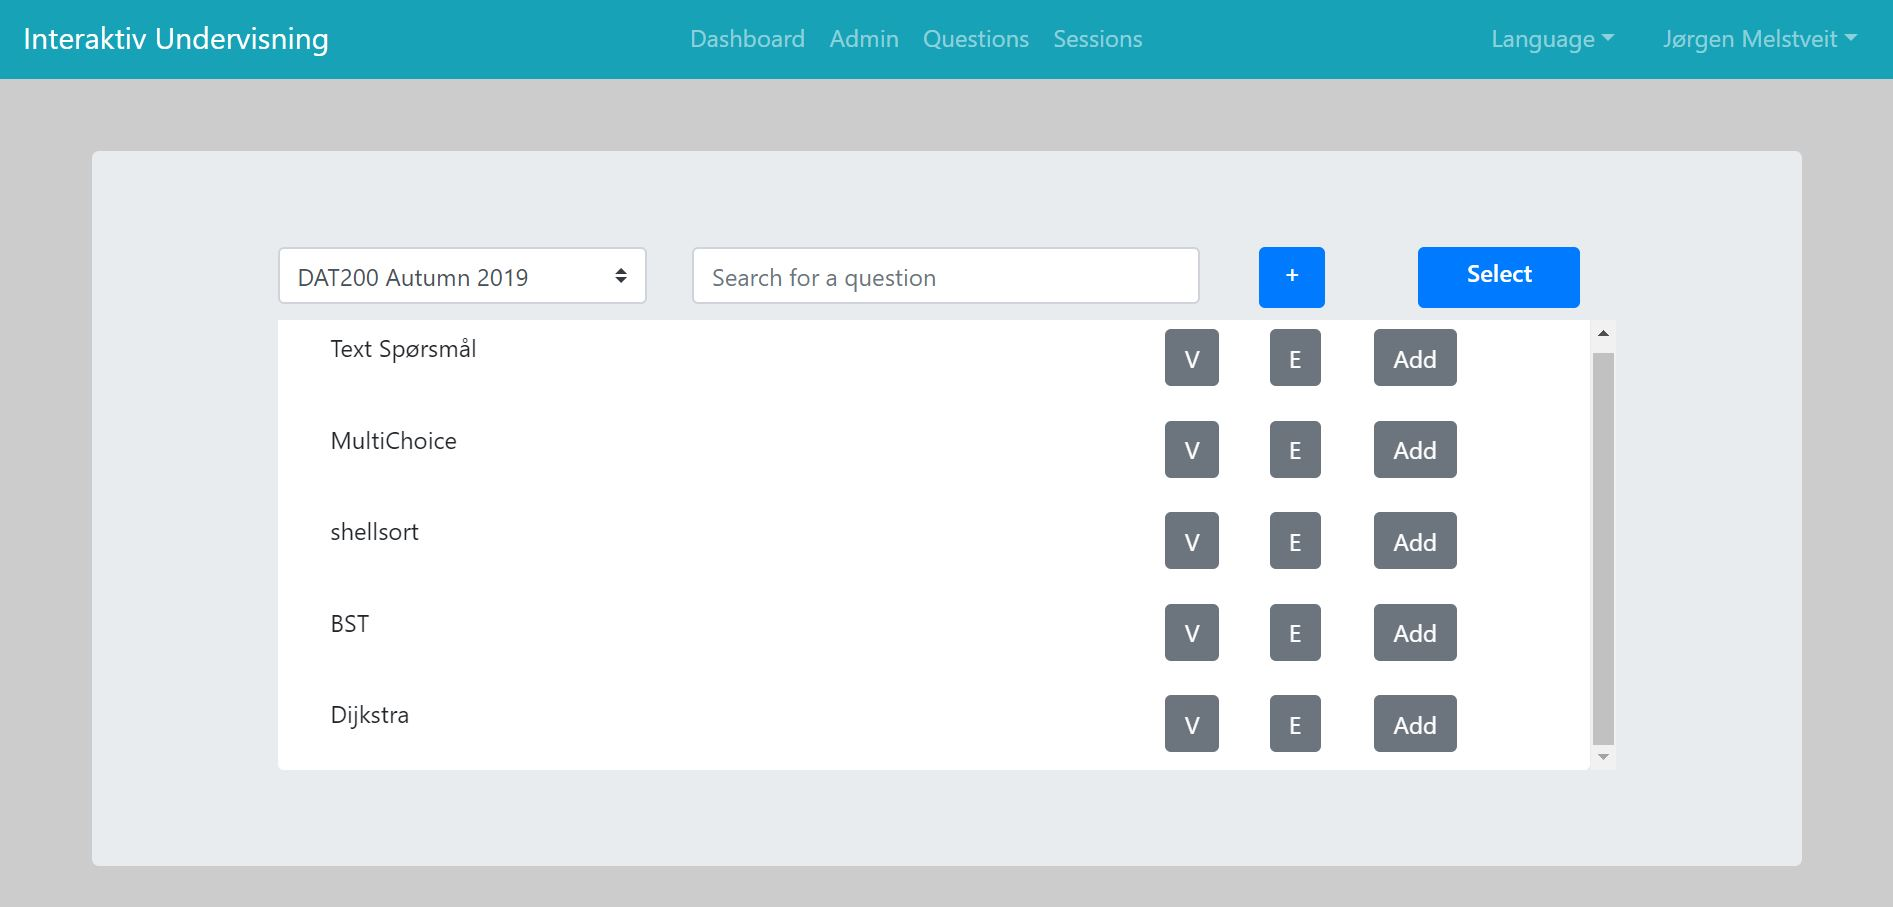
\includegraphics[width=0.80\linewidth]{/createQuestion/questionvueEnglish}
	\caption{The figure displays an image of the Questions.vue. This is the component is primarly used for allowing users to create new questions for a selected course. }
	\label{fig:questionVue}
\end{figure}
\noindent
To create a new question the user first needs to click the button with the label “+”. This will reveal the EditQuestion component which contain a vue-modal element that has all the needed forms needed for creating a question. EditQuestion is a component that is used for both adding new questions and editing existing questions. The main differences between the add and edit operations for the component are the following:
\begin{itemize}
\item[-] The title of the modal will be different. Either its going to be “New Question” for the add functionality or “Change Question” for the edit functionality.
\item[-] The edit functionality needs to load the question data from the database and fill in the forms with the correct information. 
\item[-] The request sent to the server with the question information are different. The server requests are different primarily to distinguish between the insert and update SQL commands used on the database.
\end{itemize} 
Originally there were 2 components used for the two operations, but this was later changed in development because having 2 components that were practically the same was deemed unnecessary. The modal in EditQuestion is divided into 3 parts, namely Basic Information, Media and Solution type.  These parts can be opened and closed to the user’s preference, where basic information is open by default and the other parts will be closed. Basic Information part contains an input field for assigning the question title, a textarea for giving the question a description, a time input field and a time slider. The input field is used for giving the question a title. The textarea and the time slider are both using v-model to mount to the variables newquestion.description and time respectively. These can be found in the intializeState function. This is done so that data in these fields are relatively easy to acquire and keep track of. The time input has a watcher that checks for changes to the variable that the time slider is mounted to. This means that these elements always changing their value dependent on the other, resulting in them having the same value. If the time is set to “00:00”, then the question will not have a timer when used in a session.
\\[11pt]
The media part is an optional part and is not required to be used to make a new question. The “Media” part on the EditQuestion component consists of a select box, and a part that will display added media at the bottom. The select box is used for choosing the wanted media type. Once the select box has the value “images”, the media part is set up for adding images to the question. This in turn will make a button appear with the text “Choose a file to upload...”. This button is used for adding an image to the question. Once the button is clicked the file browser will be displayed for the user and allow them to choose an image on their computer and put it onto their question. Once the image is chosen, the EditQuestion component will take the image and then validate the image given. It is important to check that the file taken was an actual image file. If the validation passes, then the image is turned into a buffer. When the question is going to be saved on the database, the question will also contain the file paths to the images given to the question. The buffer is then sent to the server and is turned back into an image. Now that the buffer is removed the path to the image is stored in the database. Whenever a question is obtained from the database that has images, the server will collect the images by using the routes stored with the question. When the image is going to be used on the client again the image will be transformed back into a buffer. A question cannot have to many images assigned to it, as this would take up a lot of the needed data. The total amount of files attached to a question cannot exceed 1.5MB, and the user will get a warning once the amount exceeds 500KB. Theses checks will run in the validation once a image is added to the question. Once an image is added to a question it will be displayed as a preview with filename, file size and a small preview imagenon the side.
\\[11pt]
Another media that is available to add to a question is tables. Once the tables is selected from the media selector, a window for editing a table appears. This window contains buttons to add/remove rows and columns. Each cell contains an input field to add a value. After a table have been saved to a question, it appear as a preview at the bottom, where the user is able to see all the added tables and what they contain. The last media that is possible to include is a graph made with the GraphDrawer. This feature allows the user to draw with the GraphDrawer and save the canvas as an image. This image is also added to the overall image sizes. So a combination of graphs and images can't exceed 1.5MB. When running a session, a question contains only media that the user uploaded, drew using the GraphDrawer, or tables.
\\[11pt]
The solution type part focuses on setting the question type to the new question and for creating the questions solution. The type will control what format the question will have for both the solution and for the client during a session. Most of the question types available are usually centered around a data structures or an algorithm from the Dat200 or Dat100 courses. There are also normal question types like multiple choice and text questions. The question type chosen will alter the available options in the solution type, so that the user can fill in the information needed for the chosen algorithm or data structure. For instance, Binary Search, AVL, Python and Dijkstra question types all require the GraphDrawer tool. The solution for questions revolving data structures and algorithms are created on the server in the solution generator. The user only needs to apply the necessary information for the question so that it is possible for the student to solve it, and for the server to be able to create the solution. As stated, before the necessary information needed for the question is determined by the question type. The are 2 reasons for having the server handle the solution. The first reason is to keep it away from clients participating in a session. The second reason is because forcing the user write the entire solution in every question would be rather tedious for the admin user. Not to mention reducing the chances of having the solution being written incorrectly.
\begin{figure}[H]
	\centering
	\begin{subfigure}{0.70\linewidth}
		\includegraphics[width=\linewidth]{/createQuestion/editQuestionUnopenedEnglish}
		\caption{This figure displays an image of the EditQuestion component when all the 3 parts Basic Information, Media and Solution type are hidden. Clicking on the labels would reveal the content of chosen part.}
		\label{fig:editquestionUnopened}
	\end{subfigure}
	\begin{subfigure}{0.70\linewidth}
		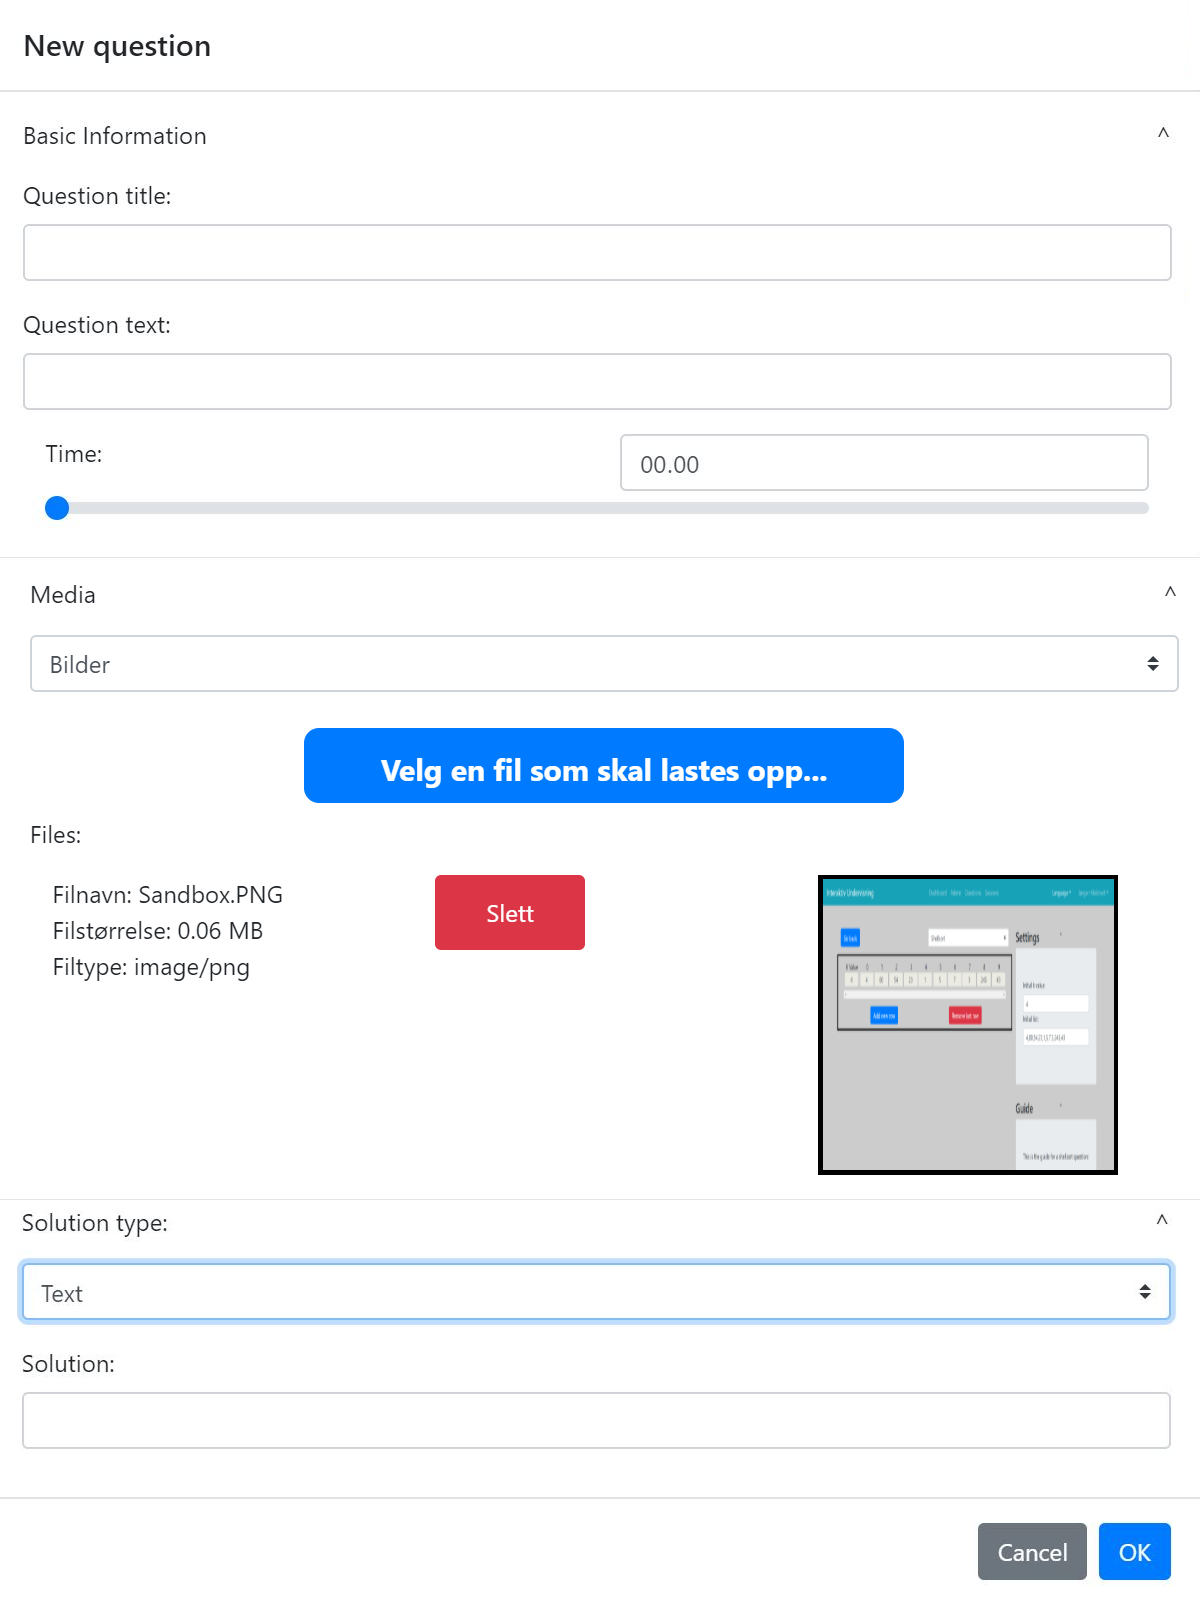
\includegraphics[width=\linewidth]{/createQuestion/editQuestionCombined}
		\caption{This figure displays an image of the EditQuestion component when all the 3 parts Basic Information, Media and Solution type are displayed. Clicking on the labels would hide the content of chosen part.}
		\label{fig:editquestionOpened}
	\end{subfigure}
\end{figure}
\noindent
Once the question is finished the question information will be sent to the server through a socket emit request. The data sent to the server is the newQuestion object found in the function initializeState() in the EditQuestion component. Since all the variables in the newQuestion object are linked to the EditQuestion component, the server should have all the information it needs for the questions solution to be created. However, to avoid any problems regarding storing faulty questions on the server, the question information will first need to be validated by the server's validation checker. The user must at minimum fill in the information in basic information and solution type for the wanted question to be valid. The question information sent to the server will first be validated on the basic information in the question. After that, if the question has an attached media to it then it is validated next. Finally, another validation test that is determined by the given questions type. Pretty much all the question types have their own unique check in the validation checker which are separated in different JavaScript files. If validation checker returns false, then the question failed the validation criteria and the errors given by the validation checker will be returned to the EditQuestion component as an alert box. The errors received by the validation can be vary, but all error message that were triggered will be shown to the user in the alert box. The text shown in the alert box for each error message from the validation checker are stored in the locale files. If the validation succeeds, then the information is sent to the solution generator that generates the appropriate solution in accordance to the questions type. The solution generator has structure similar to that of the validation checker. Each solution generator has its own JavaScript file. The main SolutionGenerator.js file is used to link the question to its appropriate solution generator function. If the question requires the GraphDrawer tool to visualize its solution, then the solution object created from the generator is going to follow a certain format. The solution object here is   an array that contains all the steps necessary to solve the exercise marked with a type variable assigned with the action taken at the step. The last step is going to indicate either “finish” or “done” and is always going to be the last entry in the array. It is this object that is going to be used in the solution checker during an active session. The reason why this structure is used for solution using the GraphDrawer, is because the GraphDrawer has ability to show the entire process of solving the chosen exercise revolving an algorithm or a data structure. However, the GraphDrawer tool requires this format for this to work.  Once this is done, the question information and solution are inserted into the question table in the database. After the question is stored in the database, the EditQuestion component is closed, and the user is returned to the Questions component. The Questions component is then going to update its question list to accommodate for the changes done on the database.
\\[11pt]
Once a question is created and is listed on the Questions component, there will be more options available for the user regarding the question. The button with the drawing symbol label will open EditQuestion component and let you edit the information previously saved for the question. Do keep in mind that the changes to the existing question are not going to be saved unless a new request is sent to the server. This means that the new question info given must also be fully validated by the validation checker, and a new solution needs to be created for the solution generator to overwrite the previous solution. If the validation fails, then the edits will not be saved in the database. It is also not possible to edit a question type once it has been assigned to a session. Once a question is assigned to a session, it will have its status to change to active. This is indicated on the question on the Questions component when the edit button has a grey background. The reason for not allowing any question to be altered after it has been assigned to a session is because it would affect the saved data after a session is finished. Which means that when a question has been assigned to a session, then that question is deemed finished by the application and can should no longer be altered.
\\[11pt]
The button labelled the eye symbol causes the component ShowQuestion to become visible. This component will load in all the information regarding the chosen question. The ShowQuestion consist of a v-modal that has similar design to the EditQuestion component. Its divided into the same three parts as the EditQuestion, where Media is only shown in the component if any images, tables or graphs are included in the question. In the basic information section, the user can view the basic information of the question like title, description and the time limit. In the media section, the user can view all the images, tables or graphs currently linked to the question. This includes information about the file such as name, type and the size. In the solution section the solution for the question will be displayed. What is shown is dependent on the solution type. Text, Multichoice and Binary tree will show the answer/answers in plain text. Every other question type will use the GraphDrawer tool to display the solution. 
\begin{figure}[H]
	\centering
	\begin{subfigure}{0.80\linewidth}
		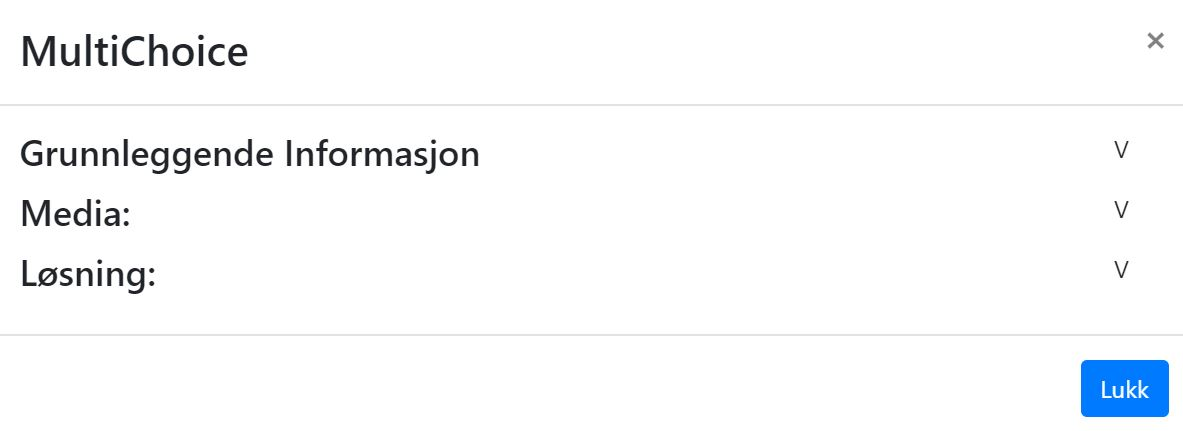
\includegraphics[width=\linewidth]{/createQuestion/showQuestionEnglishUnOpened}
		\caption{This figure displays an image of the ShowQuestion component while all the 3 parts are closed. Clicking on the labels should open op the chosen part.}
		\label{fig:showQuestionUnOpened}
	\end{subfigure}
	\begin{subfigure}{0.32\linewidth}
		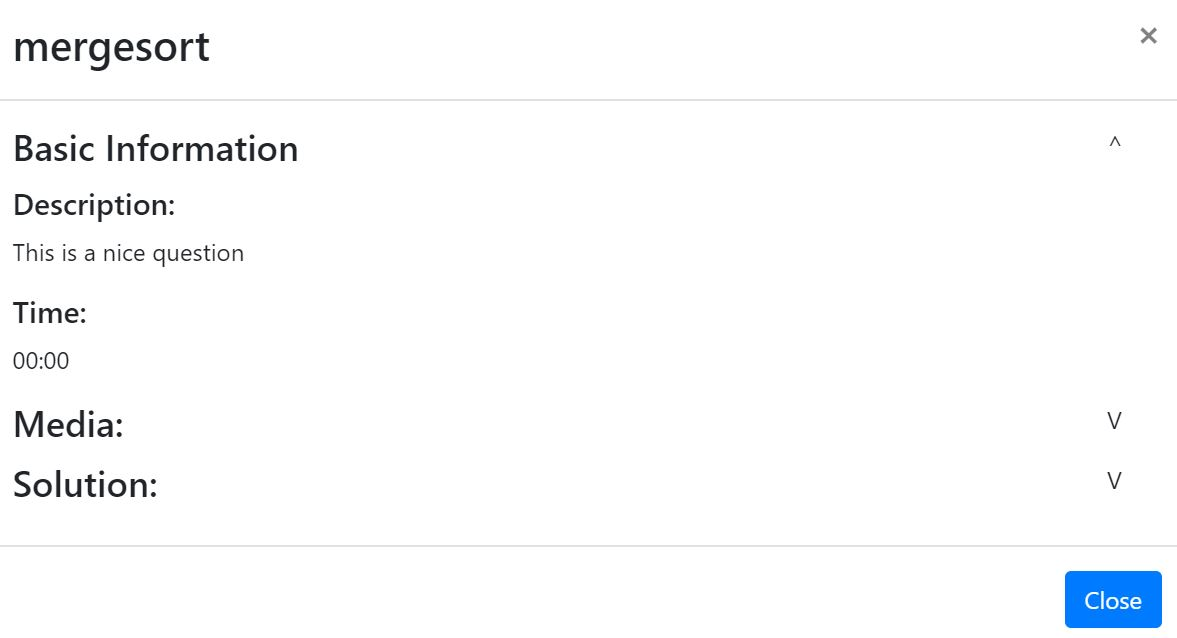
\includegraphics[width=\linewidth]{/createQuestion/showQuestionEnglishBasicOpened}
		\caption{}
		\label{fig:showQuestionBasicOpened}
	\end{subfigure}
	\begin{subfigure}{0.32\linewidth}
		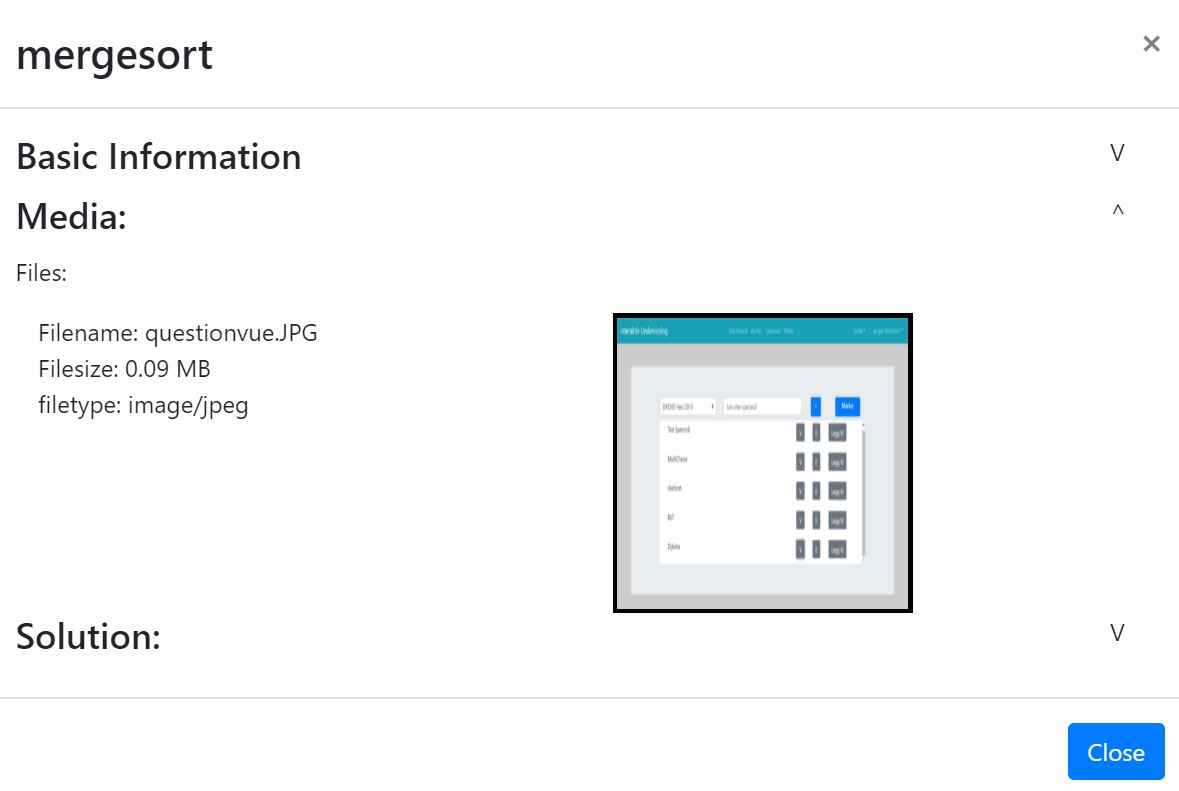
\includegraphics[width=\linewidth]{/createQuestion/showQuestionEnglishMediaOpened}
		\caption{}
		\label{fig:showQuestionMediaOpened}
	\end{subfigure}
	\begin{subfigure}{0.32\linewidth}
		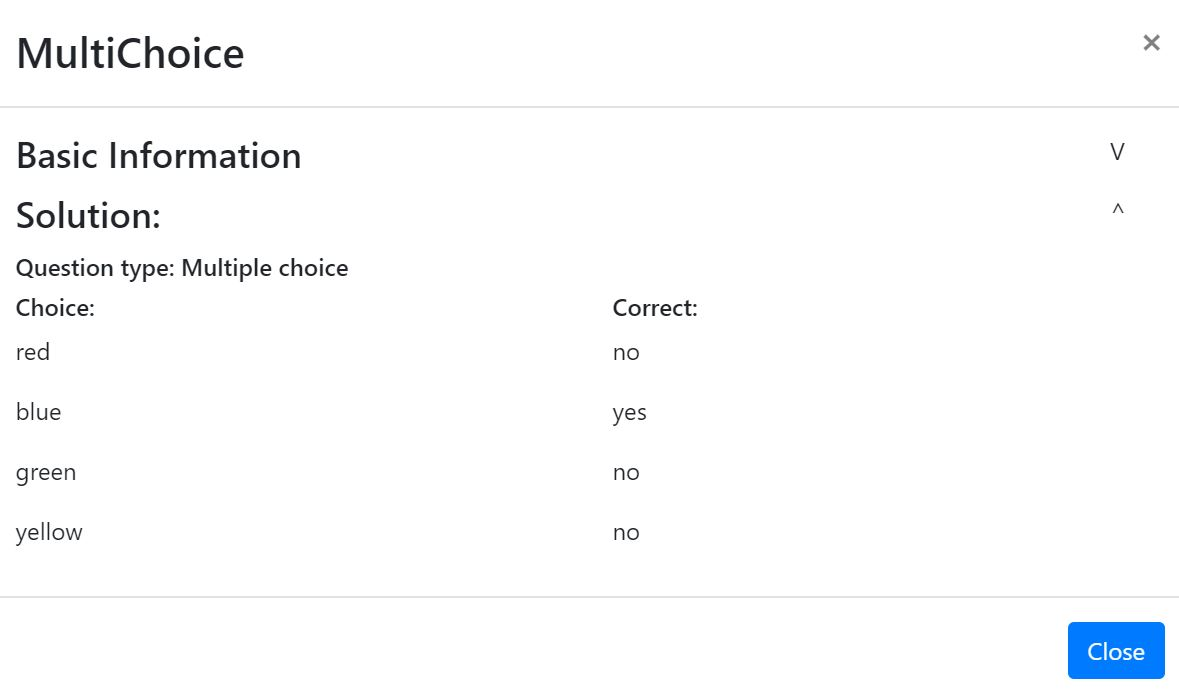
\includegraphics[width=\linewidth]{/createQuestion/showQuestionEnglishSolutionOpened}
		\caption{}
		\label{fig:showQuestionSolutionOpened}
	\end{subfigure}
\end{figure}
\noindent
The last button labelled Add will show the addQuestionToSession component. This component will only display a select box containing all current available sessions in the database. The user can select box one of these sessions and add the chosen question to the chosen session in the select box. This was implemented to give admins the options of adding more questions to an existing session, without having to create an entirely new session just for adding an extra question.
\\[11pt]
Lastly the Questions component allows you to mark question in the list by clicking on the button with the label “Select”. Once the button is used, the user has the option of either copy the selected questions to another course or deleting the questions from the current course. When a question is copied an identical question is created where the course id foreign key is assigned to the chosen course and is stored in the database. When a question is deleted, the question is simply deleted from the database. To exit the select mode simply click on the select button again, which now has the label “Close”. The copy button will use the CopyQuestions component while the delete button will use the DeleteQuestions component. If the user attempts to copy or remove without having selected a question, then an alert box will appear stating that there are no questions currently selected. Keep in mind that it is not possible to remove questions from a course if its already been used in a session. The reason for this is that the question information is still needed for Feide users to look at their previous participated sessions. If the question were to be removed after having been used in a session, then the student wouldn't have access to the question information. Therefore, the students would have no way of looking at their old session results. 
\\[11pt]
The question structure for this application was specifically chosen in a way it would be easier for developers to implement and add new questions types. Excluding the work that is needed for writing the actual data structure or algorithm and its solution format, all that is required in order for a new question type to be added to a session is the following. Create a vue component in both the questionResultScreenAnswer and questionResultScreenSolution directories. These are going to be used for DisplayQuestion component which is used for showing session results after each question. Next add a b-form-group to the EditQuestion component where only the necessary form items and Graphdrawer are set so that the user can create the new question type. If the question type requires a certain unique information, then an extra variable in the newQuestion.objects in the initializeState function should also be assigned and modeled appropriately to the html element in the form group. Then add a JavaScript file in the validation checker for stopping illegal actions to the new type. Then implement the solution generator for the question type which is going to create the format for the solution object stored in the database. Finally create a solution checker that is going to verify that the student answered the question correctly according to the solution object that was withdrawn from the database. The user may also have to update the locale files as well if some new predefined text is needed.\\[11pt]



